\documentclass[a4paper,12pt]{jsreport}
\usepackage{bm}
\usepackage[dvipdfmx]{graphicx}
\usepackage{amsmath,amsfonts}
\usepackage{physics}
\usepackage[version=4]{mhchem}
\usepackage{comment}
\usepackage{here}
\usepackage{enumitem}
\usepackage{datetime2}
\usepackage{titlesec}
\newcommand{\diff}{\mathrm{d}}


\begin{document}
\tableofcontents
\chapter{日毎メモ}

\section*{12/12(木)}
1st.texに一旦まとめることを決めた。
\section*{12/13(金)}
ls項やその他も対角成分しか持ち得ないことを今更になって気がついたため、コードを修正。
ここからはスピン$S$の取り扱いを考える。ていうかどうすればええねん。
\section*{12/14(土)}
ls項とCoulomb項を追加した。seniority pairingをどのようにすればよいのか考えながらよく使う物理定数を
まとめておこうかなと思う。上で対角成分しか持たないとか言ってたけど、拡張性を保ちたいので、結局波動関数を
Wave1,Wave2の2つ用意することで解決。$n_1=n_2,l_1=l_2$の部分のみ$E_0$が加えられるようにした。
\begin{equation}
  H_{ij}=E_0\delta_{n_1n_2}\delta_{l_1l_2}
\end{equation}
\section*{12/15-12/19}
ずっとRing Schuck読んでた。
\section*{12/20(金)}
進捗報告会で行列要素の計算に問題があることが判明した。問題を切りわけるためにHOモデル、WSモデル、WS include ls
と場合を分けながら問題点がどこにあるのかを確認しようと思う。以下、$f(r)=\frac{1}{1+\exp{((r-R)/a)}}$とする。
\begin{align*}
  H_{HO}&=\hbar \omega_0\left(2n+l+\dfrac{3}{2}\right)\\
  H_{WS}&=\hbar \omega_0\left(2n+l+\dfrac{3}{2}\right)+u_0 f(r)\\
  H_{WSso}&=\hbar \omega_0\left(2n+l+\dfrac{3}{2}\right)+u_0 f(r)+u_{ls}r_0^2\dfrac{1}{r}f'(r)\bm{l}\cdot\bm{s}\\
  H_{all}&=\hbar \omega_0\left(2n+l+\dfrac{3}{2}\right)+u_0 f(r)+u_{ls}r_0^2\dfrac{1}{r}f'(r)\bm{l}\cdot\bm{s}+U_{\text{Coul}}(r)\dfrac{1-\tau}{2}\\
\end{align*}
ここで、$U_{\text{Coul}}(r)$は一様帯電球のつくるポテンシャルである。
\begin{equation}
  U_{\text{Coul}}(r)=
  \begin{cases}
    \dfrac{(Z-1)e}{8R^3\pi\epsilon_0}(3R^2-r^2) & \text{if $r<R$,} \\
    \\
    \dfrac{(Z-1)e}{4\pi\epsilon_0r}& \text{if $r>R$.}
  \end{cases}
\end{equation}
\section*{12/21(土)}
上のコードを具体的に書いた。スピン相互作用は愚直に成分を書き表したほうが早そうだった。
自由度を結局$n,l,s$の三成分にした。それに伴い、ハミルトニアンのインデックス$H_{ij}$の割当をいい感じにした。
$i=((n\cdot N_l)+l)\cdot N_s+s$ここで、$n,l$のそれぞれの最大値(上限)を$N_{max},l_{max}$としたとき、
$N_l=l_{max}+1,N_s=2$である。
もともとの3次元調和振動子の波動関数$\psi_{nlm}$について、
\begin{equation}
  \int\psi^{*}_{nlm}\psi_{n'l'm'}d^3r=\delta_{nn'}\delta_{ll'}\delta_{mm'}
\end{equation}
\section*{12/22(日)}
\section*{12/29(日)}
Juliaでコードを組み直してみたら簡単にいい感じになってびっくりした。計算結果があってるか確認したい。
seniority modelについて着手するために色々考えていたが、
量子数はunpair中性子数$s$とj-殻の最大ペア数$\Omega$をとれば良い感じにできそうだと考えた。
\section*{2024-12-30}
seniorityの進捗をうもうとして色々考えた。特に何も生まれなかった。
\subsection*{内容}
倍といったあとにボウリング行った。楽しかった。
\subsection*{反省}
seniorityの進捗をうもうとして色々考えた。特に何も生まれなかった。
\subsection*{次の日にやること}
大晦日なのでなし。
\section*{2024-12-31}
\subsection*{内容}
LoL収めしようと思ったのにADCしかやれなかった。クソゲーすぎる。
\subsection*{反省}
苦手ロールでもどうにかなるようにしたい。
\subsection*{次の日にやること}
お正月なのでメインは休みます。
\section*{2025-01-01}
\subsection*{内容}
LoLしてた。シンジドjgたのちい
\subsection*{反省}
研究一ミリもしなかった。
\subsection*{次の日にやること}
帰省するからそこそこ頑張る。
\section*{2025-01-06}
\subsection*{内容}
卒研は進んだ。が、radial関数が悪さして$2s_{\frac{1}{2}}$がうまく表現されていない。
面倒だったので、全部ChatGPTに投げたらどうにかなったし、C言語でも困ってたところだったので助かった。
\subsection*{反省}
流石にChatGPTに頼りすぎているかもしれないが、せっかく課金してるんだしこれくらい使わせろって話。
\subsection*{次の日にやること}
seniorityの進捗を生みながら、BCSの調査を行う。
\section*{2025-01-08}
\subsection*{内容}
seniority modelを考えるときに必要なギャップ$\Delta=\dfrac{1}{2}(E_{g.s.}^{(N+1)}+E_{g.s.}^{(N-1)}-2E_{g.s.}^{(N)})$を
結合エネルギーとgrand stateの関係$E_{g.s.}^{(N)}=-B(N)+Const.$より、質量差から求める。平均的に$\Delta\simeq12/A^{-\frac{1}{2}}$であるから
これを用いてなんとなくの確認を行う。\par
BCSパラメータである$v_k$に対する拘束条件$2\sum_{k>0} v^2_k=N$を用いて化学ポテンシャル$\lambda$を求める。\par
$v^2_k=\dfrac{1}{2}\left(1-\dfrac{\epsilon_k-\lambda}{\sqrt{(\epsilon_k-\lambda)^2+\Delta^2}}\right)$を代入することで数値的に解くことを用いる。
ニュートン法を使って非線形なものを解く。$F(\lambda)=\sum_{k>0}\left(1-\dfrac{\epsilon_k-\lambda}{\sqrt{(\epsilon_k-\lambda)^2+\Delta^2}}\right)-N$として
$F(\lambda)=0$になるような$\lambda$を求める。いい感じに全部の定数を計算できたと思ったらNと整合しなくて困っていた。
実際は$\lambda$の範囲を適当にやってしまっており、物理的に($-9.81\leq \lambda \leq -7.85 $)を満たさなければならないのに、良くないところにいた。
\subsection*{反省}
特にない。
\subsection*{次の日にやること}
有限温度のBCS modelを導出する。
可能ならTeX打ちしたあとにコードも作成したい。
\section*{2025-01-09}
\subsection*{内容}
有限温度のBCSの導出ができた。
ペアリングの強さを求めるときに
Fermi分布が入り込むこと以外は絶対零度のBCSと同じ流れではあった。
\subsection*{反省}
昼に起きちゃった。。。
\subsection*{次の日にやること}
進捗報告会で無事に生き残ること。
\section*{2025-01-10}
\subsection*{内容}
有限温度のGap方程式が、
\begin{equation}
  \Delta = \dfrac{G}{2}\sum_{j} \dfrac{\Delta}{\sqrt{(\epsilon_j-\lambda)^2+\Delta^2}}\tanh(\dfrac{1}{2}\beta(\epsilon_j-\lambda)) 
\end{equation}
で与えれられることを導けた。
ここからは自明な解である$\Delta=0$以外の解がなくなるような温度$T_c$と
その時のgapの$\Delta_{T}$
を求める。
\subsection*{反省}

\subsection*{次の日にやること}

\section*{2025-01-12}
\subsection*{内容}
有限温度のBCS理論について、条件などを整理することでどの式を用いて何を求めるのかを整理した。
それによってどの方程式を用いて計算すればよいのか明確になった。
それを行った結果計算がうまく出力できてワロタ。(図\ref{FTBCS})

\subsection*{反省}

\subsection*{次の日にやること}

\section*{2025-01-24}
\subsection*{内容}
gap方程式が間違ってた。$\tanh$の中が間違っていた。$\beta\sqrt{(\epsilon_j-\lambda)^2+\Delta^2}$にせにゃいかん。
\subsection*{反省}
熱力学の復習してね♡有限温度の導出の復習をするべきやね。
\subsection*{次の日にやること}
独立にグランドポテンシャルの計算を行い、相転移が起きているということを図示したい。
$G$はそのままに$\lambda$を求めれば他の核でも比較できる。

\chapter{コード進捗}
\section{単粒子状態エネルギー}
単粒子状態のエネルギーは求められた。これを.txtに出力することでseniority modelの
$\epsilon_j$として取り込む。
\section{gの決定}
Binding energyからgapを求める。
その後に$v_k$の拘束条件$2\sum_{k>0}v_k^2=N$から化学ポテンシャル$\lambda$をニュートン法で求めた。
このときに、方程式の形をplotして0点になりそうな部分の周りでNewton法を回す。
そうして得られたパラメータで拘束条件を満たすか確認して整合性の確認を行って問題なかった。
\section{pairing Hamiltonianの構築}
Hamiltonianの要件は以下である。
\begin{equation}
  H=\sum_{j}\epsilon_j N_j -g S_+ S_-,
  -g S_+ S_- = -\dfrac{g}{4}\left[s^2 -2s(\Omega+1)+2N(\Omega+1)-N^2\right]
\end{equation}
\begin{itemize}
  \item $j$は$N=50-82$のであり、$\epsilon_j$は単粒子エネルギーである。
  \item sはseniority,未ペア粒子数である。
  \item single j-shell近似を行っているため、同核内のみでpairingが起きる。
  \item ペアリングが解ける場合は、エネルギー準位的に上の順位からほどけていく。
\end{itemize}
対角行列になるため、$E(N,j,s)$で表される。
状態としては$\ket{N,j,s}$が用いられる。\\
$\sum_j $についてはjはそれぞれのsub核として考えて、pairingもそれぞれのsub核で
$s_j,\Omega_j,N_j$を使って計算する。
\section{各熱力学的量の計算}
相転移なので流石に調べるべきという風潮。
分配関数から求めていくが、Hamiltonianがわかっているので特に苦労しない。
\begin{equation}
  Z = \operatorname{Tr}\left[e^{-\beta(H-\mu N)}\right]
\end{equation}
密度演算子から様々に発展できるので密度演算子も求めちゃう。
\begin{equation}
  D = Z^{-1}e^{-\beta(H-\mu N)}
\end{equation}
エントロピー$S$や、エネルギー$E$、粒子数$N$の期待値は、
\begin{align}
  S &= -k_B\operatorname{Tr}D\ln D\\
  E &= \operatorname{Tr} DH\\
  N &= \operatorname{Tr} DN
\end{align}
\chapter{よく使う定数}
\begin{itemize}
  \item 微細構造定数の逆数$\left(\dfrac{e^2}{4\pi\epsilon_0}\right)^{-1}=137.035999\qquad$(無次元)
  \item 換算定数$\hbar c=197.33\qquad$(fm$\cdot$MeV)
\end{itemize}
\chapter{図}
\begin{figure}[H]
  \centering
  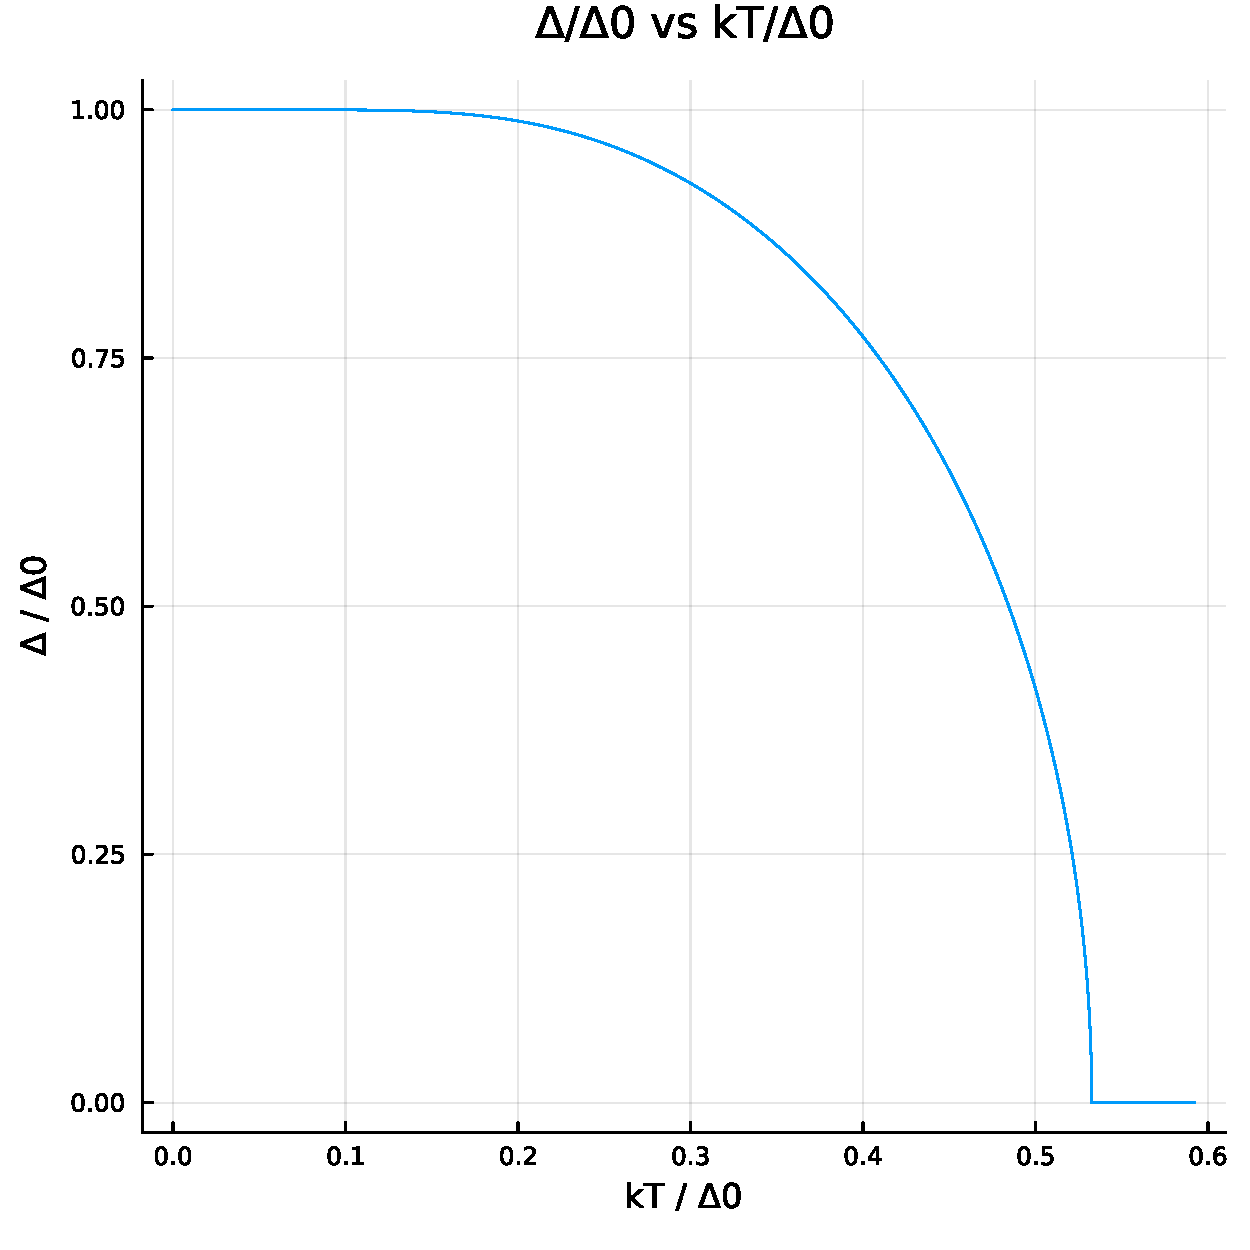
\includegraphics[width=0.8\textwidth]{FTBCS.pdf}
  \caption{Pairing gap v.s. temperature.\\ The quantity $\Delta_0$ is the gap at $T=0$.}
  \label{FTBCS}
\end{figure}
\end{document}  